\documentclass{article}
\usepackage{ctex}
\usepackage{geometry}
\geometry{top = 2cm, left = 1cm, right = 1cm, bottom = 2cm}
\usepackage{amsmath,amssymb,amsthm,amsfonts}
\usepackage{abstract}
\usepackage{siunitx}
\usepackage{graphicx}
\usepackage{booktabs}
\usepackage{appendix}
\usepackage{hyperref}
\usepackage{lscape}
\usepackage{multirow}

\renewcommand{\appendixpagename}{附录}


\title{正电子在物质中的湮灭寿命}
\author{钱思天 2001112187}
\begin{document}
    \maketitle
    \begin{abstract}
        本实验利用了多道时间谱仪,首先利用$^{60}\text{Co}$的特征峰,检查了有无能选条件下时间分辨能力。而后,利用多道时间谱仪,测量了正电子在物质中的湮灭寿命。
        \newline
        \newline
        {\emph{ 关键词:\ 多道时间谱仪、能选条件、正电子湮灭 }\rm}

    \end{abstract}

    \section{实验介绍}
    \subsection{正电子在物质中的湮灭寿命}
正电子是电子的反粒子,除电荷和磁矩符号不同外,其他特征与电子相同。当电子与正电子相遇时发生“湮没”,它们的总能量以电磁辐射能的形式发射出来。湮没过程的绝大多数是发射两个能量相等($\si{511MeV}$),方向相反的伽马光子。发射单个光子或三个光子的湮没过程,虽然可能,但几率极小。湮没过程中发射的伽马光子,通常称为湮没辐射。
放射源发射的正电子,通常具有几百keV的动能,进入物质以后,与物质的分子原子相碰撞,很快损失它的动能,在极短的时间内($\si{10ps}$)与物质达到热平衡,然后继续在物质中运动,直到与负电子相遇发生湮没。正电子从产生到湮没的时间间隔,称为正电子在物质中的湮没寿命。
   \subsection{测量正电子寿命的实验原理}
    测量正电子寿命时,正电子源通常用$^{22}\text{Na}$源。$^{22}\text{Na}$发生$\beta$正衰变时放出正电子,$^{22}\text{Na}$转变到$^{22}\text{Ne}$的激发态,此激发态的激发能为$\si{1280keV}$,寿命约$3\times10^{-12}\si{s}$秒,激发态通过发射$\si{1275keV}$伽马射线退激到$^{22}\text{Ne}$的基态。在时间谱仪的分辨时间为$10^{-10}\si{s}$秒的情况下,可认为上述核转变过程中放出的正电子和伽马射线是同时进行的。在测量正电子寿命时,$\si{1275keV}$伽马射线可作为正电子产生的时标信号,而正电子湮没时放出的两个$\si{511keV}$的伽马光子,可作为正电子湮没的时标信号。测量正电子产生和湮没的时标信号之间的时间间隔即可得正电子寿命。
\subsection{多道时间谱仪}
多道时间谱仪又被称为多道时间分析器,是测量两个时间关联事件之间的短时间间隔的装置。它可以用于测量正电子在物质中的湮没寿命,粒子飞行时间谱,核激发寿命等。
本实验中要介绍的是时幅变换器型的多道时间谱仪。它通过时间幅度变换器把关联事件的时间间隔变换成电压脉冲幅度,然后由多道分析器测量幅度分布谱,从而得到关联事件的时间分布谱。如果关联事件是原子核能级A,B,C之间的跃迁发射的级联伽马射线1和2,那么,原子核能级B的寿命可通过测定1和2之间的时间间隔得到。
\begin{enumerate}
    \item 探头:由快塑料闪烁体和快光电倍增管组成,用来探测关联事件1和2。光电倍增管的阳极负信号作为事件发生的时标信号,直接耦合到时间道的定时甄别器输入端;光电倍增管的打拿极正信号作为能量选择信号,经射极跟随器输出到能量道。共有两个探头,与每个探头相连的其它部分是左右对称的。
    \item 快道:又称为时间选择道,从时间关联关系上来选出关联事件对1和2,同时把1和2之间的时差变换为脉冲幅度。
    \item 慢道:又称为能量选择道,为了减少偶然符合本底和改善分辨时间,必须通过能量进一步选出关联事件。
    \item 快慢符合:将慢符合单元的输出信号去开时幅变换器的选通门,使时幅变换器的变换脉冲得以输出。这样时幅变换器输出的信号表示经过时间选择和能量选择的关联事件,时幅变换器输出信号的幅度谱表示关联事件2相对于1的时间谱。
\end{enumerate}
\section{实验步骤}
\subsection{实验步骤}
\begin{enumerate}
    \item 连接线路。打开一体化多道分析仪BH1324,进入微机多道数据采集程序PHA1.8。
    \item 放上$^{60}\text{Co}$放射源,调节探头1和2的工作电压(约$\si{1780\V}$,探头1高压量程取为2kV,高压调节钮读数8.9。探头2高压为1500V+300V),使康普顿谱半高约在700至900道。
    \item 调节1路和2路单道的阈值和道宽,用1024多道选择能量窗口,使。(提示:将单道输出信号作为反符合测量信号接入BH1324的“COIN IN”端,注意在接入前要将信号展宽)
    \item 用延迟插件对谱仪进行时间刻度;延迟时间分别取为16,20,24,28,32ns五个点。各插件工作条件:恒比定时都用1档,负输出;1路低阈取0.4,2路取0.2。时幅变换器时间量程用0.05us,幅度量程用1或2档,放大粗调1.0,细调1.0(旋钮读数5.0);内选通(int);负脉冲输入,正脉冲输出。
    \item 在符合单元中,固定2路延迟时间为3us,改变两路信号的相对延迟时间,测量曲线并做图。每次计数时间取30秒。确定最佳延迟时间。
    \item 延迟时间取16ns,将符合输出信号作为能选信号输入时幅变换器的“选通”(strobe)端,将选择钮拨向外选通(exit)。测量有能选情况下的钴60的瞬时符合谱,与无能选时的瞬时符合谱(在时间刻度时已做过)比较,确定两种情况下相应的分辨时间,并说明能选对分辨时间的影响。
    \item 换上$^{22}\text{Na}$源:分别选择慢道的1275keV伽马(取)和511keV伽马(取)能谱的能量窗口。
    \item 测量正电子的湮没寿命;测量时间约5000秒。拟合出长,短两个寿命;长寿命取30-40道数据,短寿命取大约20道数据。
\end{enumerate}
\section{实验数据处理}
\subsection{时间刻度曲线}
测量不同延迟时间的$^{60}\text{Co}$符合谱如图\ref{fig:time}。

\begin{figure}[htbp]
    \centering
    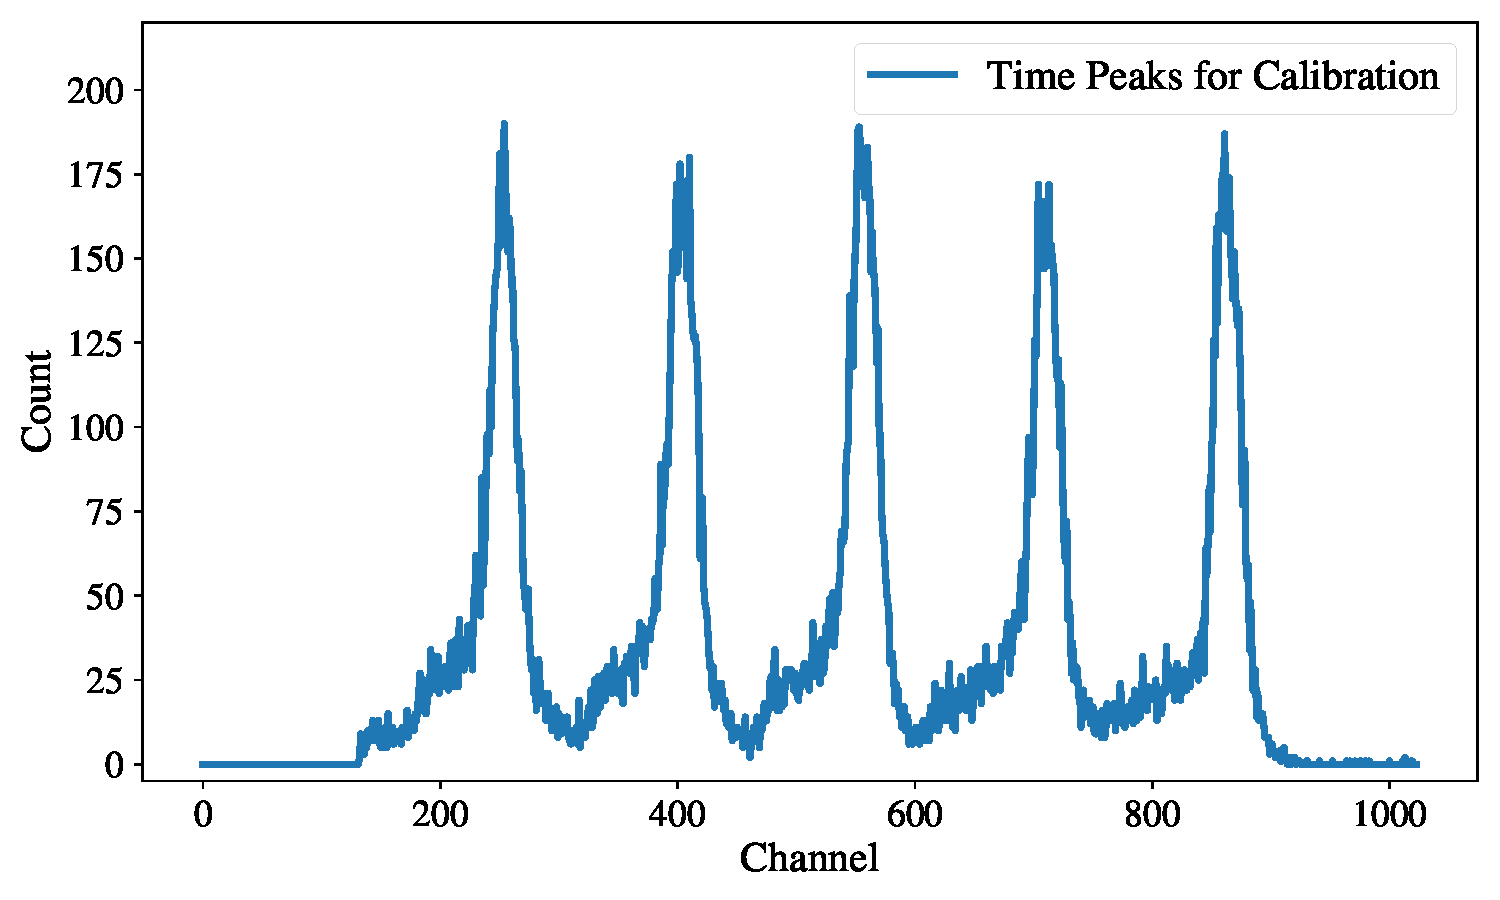
\includegraphics[width = 0.7\textwidth]{../plots/time.pdf}
    \caption{不同延迟时间的$^{60}\text{Co}$符合谱\label{fig:time}}
\end{figure}
得到不同延迟时间和峰道址位置表如表\ref{tab:time}。
\begin{table}[htbp]
    \centering
    \caption{不同延迟时间和峰道址关系表\label{tab:time}}
    \begin{tabular}{lrrrrr}
\toprule
Peak Position &  254 &  410 &  553 &  706 &  861 \\
\midrule
   Delay Time$[\si{ns}]$ &   16 &   20 &   24 &   28 &   32 \\
\bottomrule
\end{tabular}

\end{table}

将峰位和道址进行线性拟合,可以得到
\begin{equation}
    t = 0.0265\times\text{Ch}+9.2530
\end{equation}

拟合效果如图\ref{fig:TimeCalibration}。

\begin{figure}[htbp]
    \centering
    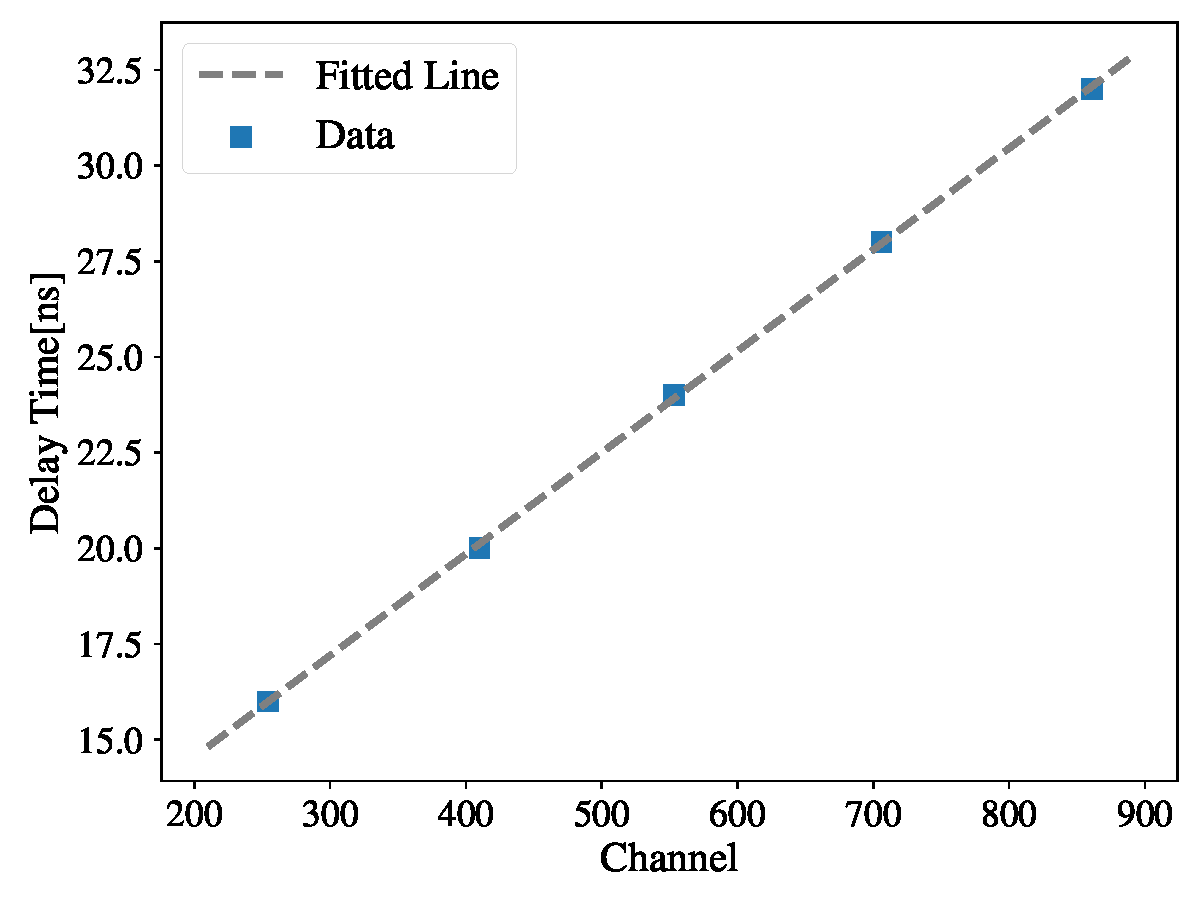
\includegraphics[width = 0.7\textwidth]{../plots/TimeCalibration.pdf}
    \caption{不同延迟时间和峰道址的关系及拟合\label{fig:TimeCalibration}}
\end{figure}

\subsection{比较有无能选关系下的峰分辨率}
有能选情况下延迟时间为$16\si{ns}$的峰如图\ref{fig:EnergySelection}。

\begin{figure}[htbp]
    \centering
    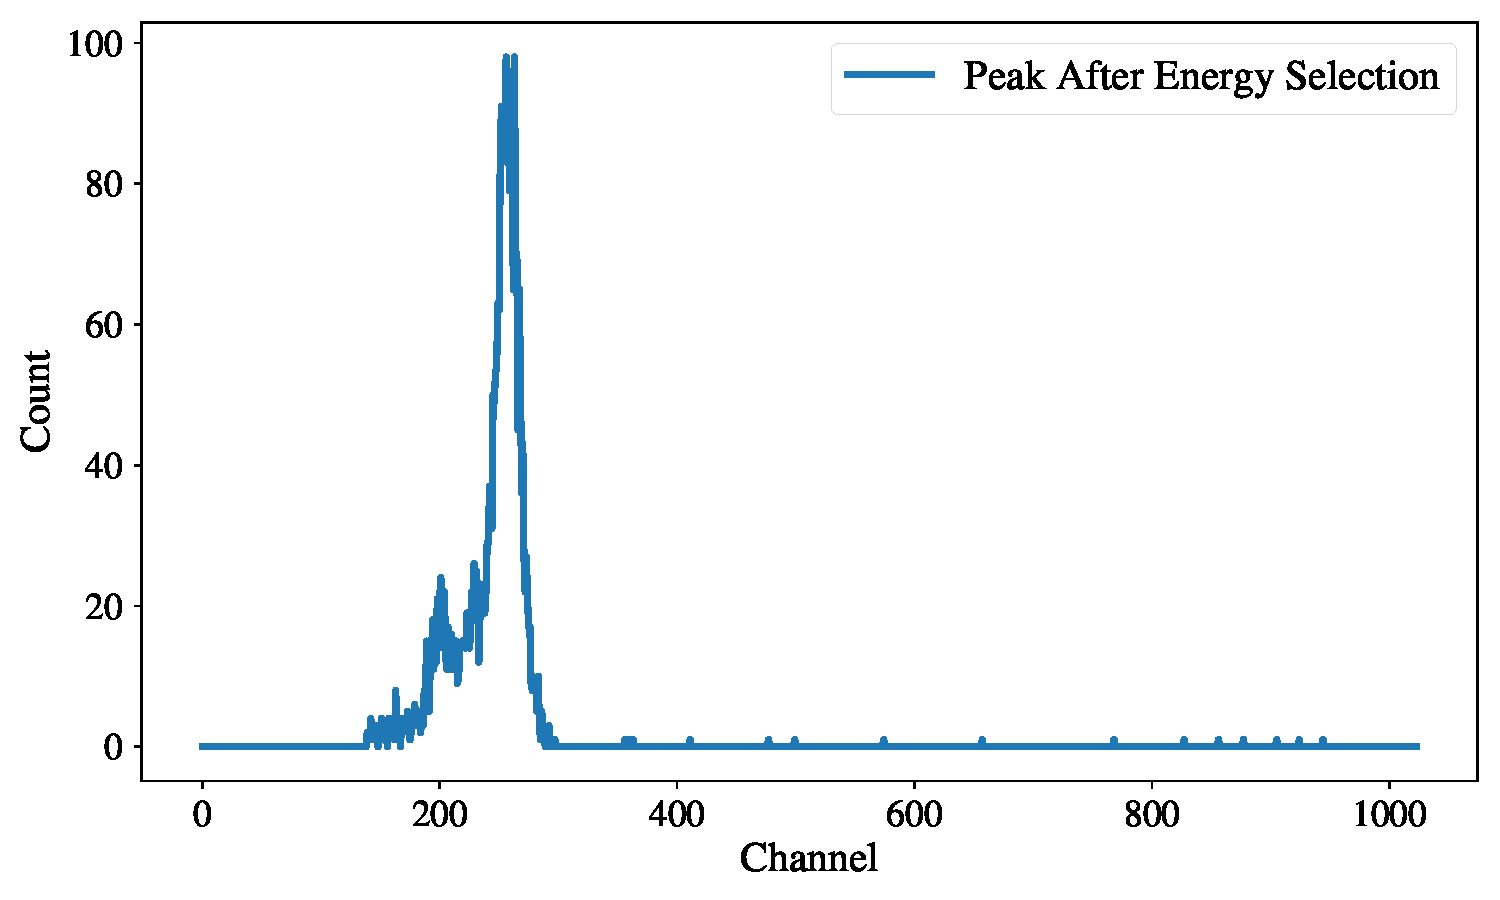
\includegraphics[width=0.7\textwidth]{../plots/EnergySelection.pdf}
    \caption{有能选条件下延迟时间为$16\si{ns}$的谱线测量结果\label{fig:EnergySelection}}
\end{figure}

对比有无能选条件下的延迟时间为$16\si{ns}$的两个峰的分辨率如表\ref{tab:EnergySelection},可见施加能选条件,可以提高测量的分辨率。

\begin{table}[htbp]
    \centering
    \caption{有无能选条件下$16\si{ns}$测量峰对比\label{tab:EnergySelection}}
    \begin{tabular}{lrrl}
\toprule
If with Energy Selection &  Peak Position &  FWHM & Resolution \\
\midrule
                     W/O &            254 &  23.5 &       9.3\% \\
                    With &            256 &  20.0 &       7.8\% \\
\bottomrule
\end{tabular}

\end{table}
\subsection{$N_c-t_d$曲线}
通过变动$t_1$,固定$t_2 = 3\si{\micro s}$,得到的$N_c-t_d$曲线如图\ref{fig:Nc_td}。由图,取$t_1 = 2.8\si{\micro s}$。
\begin{figure}[htbp]
    \centering
    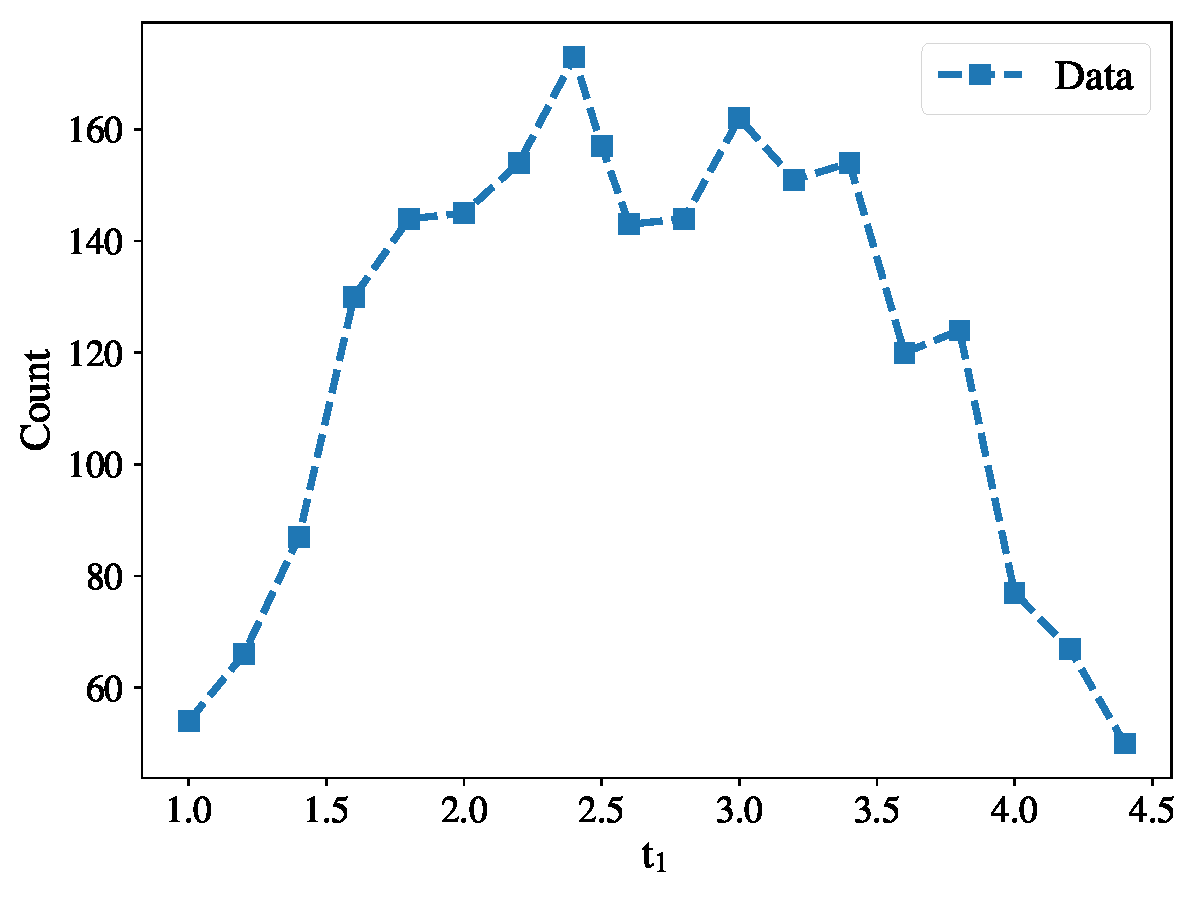
\includegraphics[width=0.7\textwidth]{../plots/Nc_Td.pdf}
    \caption{$N_c-t_d$曲线\label{fig:Nc_td}}
\end{figure}
\subsection{正电子湮灭寿命计算}
对5000s测量的谱图进行两次指数函数拟合,可以得到:
\begin{equation}
\begin{cases}
\tau_{l} = 1/0.701046 = 1.426\si{ns}\\    
\tau_{s} = 1/0.2.5822 = 0.3872\si{ns}
\end{cases}
\end{equation}
拟合结果如图\ref{fig:5ks}
\begin{figure}[htbp]
    \centering
    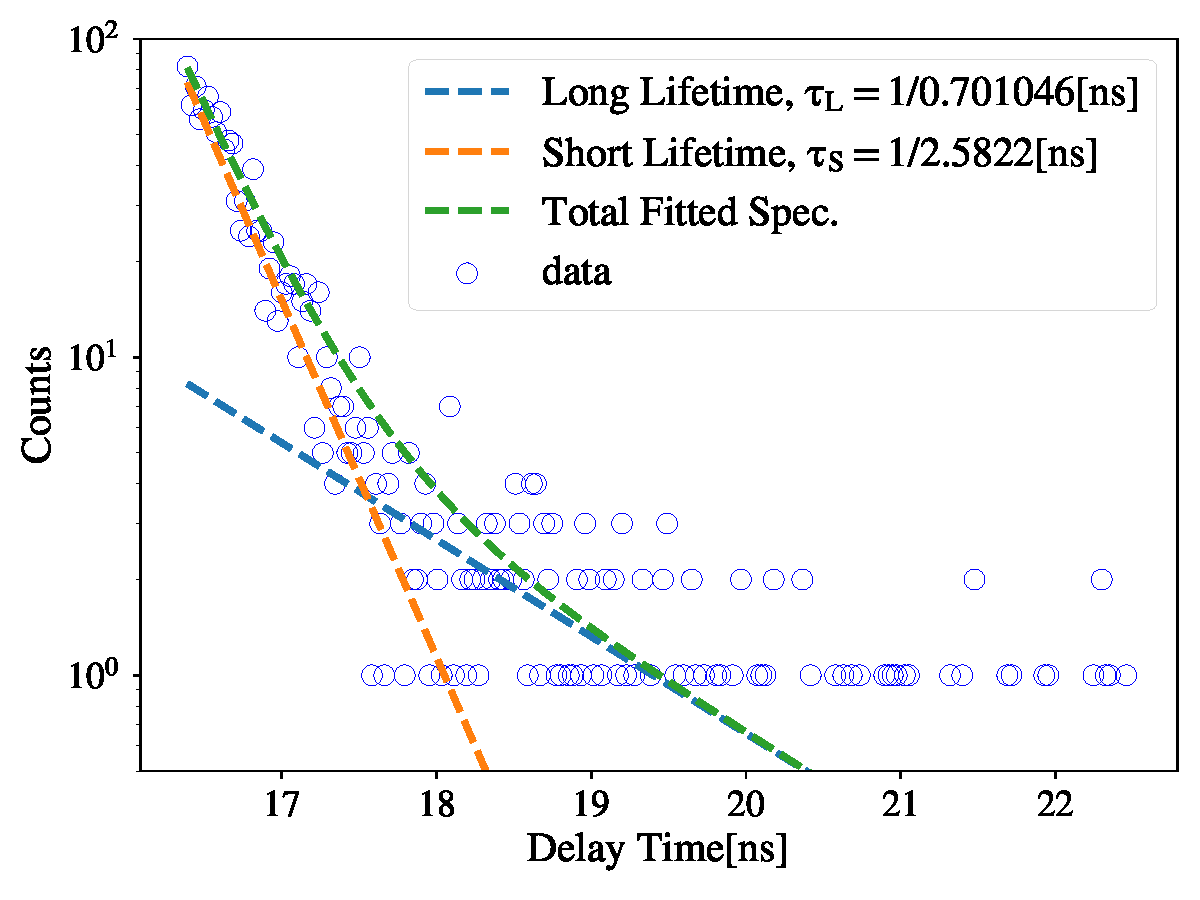
\includegraphics[width=0.7\textwidth]{../plots/5ks.pdf}
    \caption{对正负电子湮灭寿命谱的拟合\label{fig:5ks}}
\end{figure}
\section{致谢}
    感谢赵捷老师的指导,也感谢张轩豪同学和蒋沛成同学一起进行实验。 
    \clearpage
    \appendix
    \appendixpage
    \section{思考题:5-12}
    \begin{enumerate}
        \item 两束$\gamma$射线是否来自同一级联辐射的概率是一个确定的二项分布,从而在大统计量下会近似为高斯分布,同时,还需要考虑偶然符合的存在。单道能量窗口的宽度、阈值还有两个符合信号本身的宽度都会导致瞬时符合谱的展宽。
        \item 难以获得有意义的形状,因为$^{137}\text{Cs}$并没有级联的伽马谱,从而无法进行符合。
        \item 靠近零道的一个峰。
        \item 偶然符合计数率改变导致时间谱宽度改变。
        \item 正确。基本原理都是让一个电容器在时间间隔内恒流充电,这样使得充电幅度和时间成正比。
    \end{enumerate}
    \section{思考题6-5}
    \begin{enumerate}
        \item \begin{equation}
            \begin{aligned}
                E_{e^+} + E_{e^-} &= E_{\gamma_1} + E_{\gamma_2}\\
                \vec{p}_{e^+} + \vec{p}_{e^-} &= 0 
            \end{aligned}
        \end{equation}
        得到两个光子动量大小相等方向相反,为$0.511\si{MeV}/c$,能量相等,为$0.511\si{MeV}$。
        \item 谱比较简单,只有两个寿命;有伽马射线作为正电子产生和湮灭的时标信号,便于测量正电子寿命。
        \item 是一个很细的峰。会使谱线展宽,降低测量的准确性。
        \item 实验使用的$^{22}\text{Na}$源较弱,测量时间为5000s,如果能使用活度较大的源,就可以减小误差。
    \end{enumerate}
\end{document}
